\documentclass[10pt]{article}

\usepackage[margin=0.75in]{geometry}
\usepackage{amsmath,amsthm,amssymb}
\usepackage{xcolor}
\usepackage{cancel}
\usepackage{graphicx}
\usepackage{changepage}
\usepackage{circuitikz}
\usepackage{pgfplots}
\usepackage{physics}
\usepackage{hyperref}
\usepackage{siunitx}
\usepackage{fontspec}
\usepackage{relsize}
\usepackage{subfig}
\usepackage{todonotes}
\usepackage{minted}
\usepackage{multicol, multirow, booktabs}
\usepackage[breakable]{tcolorbox}
\usepackage[inline]{enumitem}

\theoremstyle{definition}
\newtheorem{problem}{Problem}
\newtheorem{soln}{Solution}

\pgfplotsset{compat=newest}
\usetikzlibrary{lindenmayersystems}
\usetikzlibrary{arrows}
\usetikzlibrary{calc}
\usetikzlibrary{positioning, fit}
\usetikzlibrary{3d, perspective}

\definecolor{incolor}{HTML}{303F9F}
\definecolor{outcolor}{HTML}{D84315}
\definecolor{cellborder}{HTML}{CFCFCF}
\definecolor{cellbackground}{HTML}{F7F7F7}
\newcommand{\ui}{\hat{i}}
\newcommand{\uj}{\hat{j}}
\newcommand{\uk}{\hat{k}}
\newcommand{\ux}{\hat{x}}
\newcommand{\uy}{\hat{y}}
\newcommand{\uz}{\hat{z}}
\newcommand{\primed}[1]{#1^\prime}
\pgfdeclarelayer{background}  
\pgfsetlayers{background,main}
\AtBeginDocument{\RenewCommandCopy\qty\SI}

\makeatletter
\newcommand{\boxspacing}{\kern\kvtcb@left@rule\kern\kvtcb@boxsep}
\makeatother
\newcommand{\prompt}[4]{
    \ttfamily\llap{{\color{#2}[#3]:\hspace{3pt}#4}}\vspace{-\baselineskip}
}

\newcommand{\thevenin}[2]{
  \begin{center}
    \begin{circuitikz} \draw
      (0,0) -- (2,0) to[battery1, l_=$V_{Th}\eq#1$] (2,2) 
      to[resistor, l_=$R_{Th}\eq#2$] (0,2)
      ;
      \draw [o-] (-.07,2.079);
      \draw [o-] (-.07,0.079);
    \end{circuitikz}
  \end{center}
}

\newcommand{\norton}[2]{
  \begin{center}
    \begin{circuitikz} \draw
      (0,0) -- (3,0) to[american current source, l_=$I_{N}\eq#1$] (3,2) -- (0,2) (2,0)
      to[resistor, l=$R_{N}\eq#2$] (2,2)
      ;
      \draw [o-] (-.07,2.079);
      \draw [o-] (-.07,0.079);
    \end{circuitikz}
  \end{center}
}

\newcommand{\highlight}[1]{\colorbox{yellow}{$\displaystyle #1$}}

\newcommand{\ti}[1]{\widetilde{#1}}

\newfontface{\Kaufmann}{Kaufmann}
\DeclareTextFontCommand{\kf}{\Kaufmann}
\newcommand{\scriptr}{\fontsize{12pt}{12pt}\kf{r}}

\newfontface{\KaufmannB}{Kaufmann Bd BT}
\DeclareTextFontCommand{\kfb}{\KaufmannB}
\newcommand{\bscriptr}{\fontsize{12pt}{12pt}\kfb{r}}

\newcommand{\bv}[1]{\mathbf{#1}}

\title{Physics 3610H: Assignment III}
\author{Jeremy Favro (0805980) \\ Trent University, Peterborough, ON, Canada}
\date{\today}

\begin{document}
\maketitle

% PROBLEM 1
\begin{problem}
Consider a particle in the infinite square well from $0<x<a$. The eigenstates and eigenvalues of the
T.D.S.E for this system are
\begin{align*}
  \psi_n(x) & =\sqrt{\frac{2}{a}}\sin\left(\frac{n\pi x}{a}\right) \\
  E_n       & =\frac{\hbar^2n^2\pi^2}{2ma^2}
\end{align*}
respectively. We also found that these states form an orthonormal set,
$$
  \int_{\mathbb{R}}\psi^*_n(x)\psi_m(x)dx=\delta_{mn}.
$$
Suppose a particle in such a well is in the following state at $t=0$:
$$
  \Psi(x,0)=A(\psi_1(x)+2\psi_2(x))
$$
\begin{enumerate}[label=(\alph*)]
  \item Find $A$ such that $\Psi(x,0)$ is normalized.
  \item Draw $\Psi(x,0)$ as a function of $x$.
  \item Where is the particle most likely to be found at $t = 0$? (Draw arrow(s) on your plot.)
  \item Where is the particle least likely to be found at $t = 0$? (Draw arrow(s) on your plot.)
  \item What is the probability of finding the particle in the left half of the well (i.e. $0 < x < a/2$)
        at $t = 0$?
  \item Find $\Psi(x,t)$.
  \item Show $\Psi(x,t)$ is normalized for all times $t$.
  \item What is the expectation value of $x$?
  \item If you measured the energy of this particle, what values might you get and what is the
        probability that you will get each of these values?
  \item What is the expectation value of the energy?
\end{enumerate}
\end{problem}
\newpage
\begin{soln}~
  \begin{enumerate}[label=(\alph*)]
    \item Here we force the integral over all space of $\abs{\Psi}^2$ to be 1 and solve for an $A$ which satisfies this. We can note
          that because we are dealing with an infinite well here the wavefunction is only nonzero within the well so we can trim down the bounds a bit,
          \begin{align*}
            1 & =\int_{0}^{a}\Psi^*(x,0)\Psi(x,0)\,dx                                                                            \\
              & =\abs{A}^2\int_{0}^{a}(\psi_1^*(x)+2\psi_2^*(x))(\psi_1(x)+2\psi_2(x))\,dx                                       \\
              & =\abs{A}^2\int_{0}^{a}\psi_1^*(x)\psi_1(x)+2\psi_2^*(x)\psi_1(x)+2\psi_2(x)\psi_1^*(x)+4\psi_2(x)\psi_2^*(x)\,dx \\
              & =\abs{A}^2\int_{0}^{a}\psi_1^*(x)\psi_1(x)+2\delta_{12}+2\delta_{12}+4\psi_2(x)\psi_2^*(x)\,dx                   \\
              & =\abs{A}^2\left[\delta_{11}+\cancelto{0}{\delta_{12}+\delta_{12}}+4\delta_{22}\right]                            \\
              & =\abs{A}^2\left[1+4\right]\implies \abs{A}^2=1/5\implies A=\sqrt{1/5}
          \end{align*}
          \todo[inline]{Why doesn't this work for $0<a\leq 3$????}
    \item ~\\
          \begin{center}
            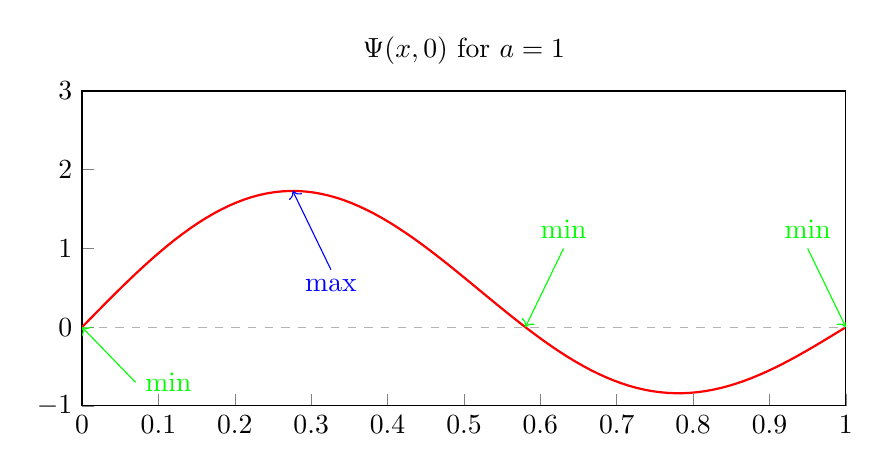
\begin{tikzpicture}
              \begin{axis}[title = {$\Psi(x,0)$ for $a=1$},
                  ymax = 3,
                  ymin = -1,
                  xmin=0,
                  xmax=1,
                  xtick pos = bottom,
                  ytick pos = left,
                  height=4cm,
                  width=0.8\textwidth,
                  scale only axis=true]
                \draw[red, thick, domain=0:1, samples=100] plot (\x, {
                    sqrt(1/5)*(sqrt(2)*sin(deg(pi*\x))+2*sqrt(2)*sin(deg(2*pi*\x)))
                  });
                \draw[black!30, dashed, domain=0:1, samples=1] plot (\x,0);
                \coordinate (MAX) at (0.27587156664462037, {sqrt(1/5)*(sqrt(2)*sin(deg(pi*0.27587156664462037))+2*sqrt(2)*sin(deg(2*pi*0.27587156664462037)))});
                \draw[blue, <-] (MAX) -- +(+0.05, -2) node[below]{max};

                \draw[green, <-] (0.5804306232551663, 0) -- +(+0.05, 0) node[above]{min};
                \draw[green, <-] (0, 0) -- +(0.07, -1.7) node[right]{min};
                \draw[green, <-] (1, 0) -- +(-0.05, 0) node[above]{min};
              \end{axis}
            \end{tikzpicture}
          \end{center}
    \item Here we take the derivative of the wavefunction $\Psi(x,0)$ and determine the turning points,
          \begin{align*}
            0 & =\frac{d}{dx}\Psi(x,0)                                                                                                                         \\
              & =A\left[\frac{d}{dx}(\psi_1(x)+2\psi_2(x))\right]                                                                                              \\
              & =A\left[\frac{d}{dx}\psi_1(x)+2\frac{d}{dx}\psi_2(x)\right]                                                                                    \\
              & =A\left[\frac{d}{dx}\sqrt{\frac{2}{a}}\sin\left(\frac{\pi x}{a}\right)+2\frac{d}{dx}\sqrt{\frac{2}{a}}\sin\left(\frac{2\pi x}{a}\right)\right] \\
              & =A\sqrt{\frac{2}{a}}\left[\frac{\pi}{a}\cos\left(\frac{\pi x}{a}\right)+\frac{4\pi}{a}\cos\left(\frac{2\pi x}{a}\right)\right]                 \\
              & =A\frac{\pi}{a}\sqrt{\frac{2}{a}}\left[\cos\left(\frac{\pi x}{a}\right)+4\cos\left(\frac{2\pi x}{a}\right)\right]                              \\
          \end{align*}
          Which will be zero when
          $$\cos\left(\frac{\pi x}{a}\right)=-4\cos\left(\frac{2\pi x}{a}\right).$$
          This is a nasty expression to solve analytically so we force a computer to do it. I used SageMath but most advanced
          CAS software (or numerical optimization techniques, as it turns out) should be able to handle this
          \begin{tcolorbox}[breakable, size=fbox, boxrule=1pt, pad at break*=1mm,colback=cellbackground, colframe=cellborder]
            \prompt{In}{incolor}{2}{\boxspacing}
            \begin{minted}[breaklines, autogobble]{sage}
                a = 1
                A = 1/sqrt(5)
                x = var("x")
                eqn = cos(pi*x/a) == -4*cos(2*pi*x/a) #
                show(find_root(eqn, 0, a/2)) # Find roots on [0,a/2] because we need to force finding the maxima on the left rather than the minima on the right
            \end{minted}
          \end{tcolorbox}
          \begin{tcolorbox}[breakable, size=fbox, boxrule=.5pt, pad at break*=1mm, opacityfill=0]
            \prompt{Out}{outcolor}{2}{\boxspacing}
            $0.27587156664462037$
          \end{tcolorbox}
          Sadly even sage can't give me a nice analytical solution here (Interestingly, the open access version of Wolfram alpha actually can) so
          we'll have to resign ourselves to using a numerical value that has to be recalculated for new $a$. See blue mark on the plot for
          where this point lies.
    \item Here we recognize that as probability is $\abs{\Psi}^2$ we lose the sign and so are looking for the smallest value. Because we have
          points where we cross zero those will remain the smallest even when taking the modulus and squaring it and so we can look for points
          $$\Psi(x,0)=0.$$
          This are given by
          $$A\sqrt{\frac{2}{a}}\left[\sin\left(\frac{\pi x}{a}\right)+2\sin\left(\frac{2\pi x}{a}\right)\right]=0$$
          which reduces to
          $$\sin\left(\frac{\pi x}{a}\right)+2\sin\left(\frac{2\pi x}{a}\right)=0.$$
          which we can see will have ``cheap'' solutions at $x=a$ and $x=0$. We expect from the graph however there to exist a third solution somewhere between
          these two. To find this we can again employ our CAS approach as before while restricting the solver to between $0+\epsilon$ and $a-\epsilon$ where
          $\epsilon$ is sufficiently small that the algorithm (whatever you chose) will skip the trivial endpoints. Doing this for our case of $a=1$ gives
          $x=0.5804306232551663$. This is, and the other two points, is marked in green on the original plot.
    \item Here we just integrate our probability density over $0\to a/2$,
          \begin{align*}
             & P(0<x\leq a/2)=\int_{0}^{a/2}\abs{\Psi(x,0)}^2\,dx                                                                 \\
             & =\int_{0}^{a/2}A\sqrt{\frac{2}{a}}\left[\sin\left(\frac{\pi x}{a}\right)+2\sin\left(\frac{2\pi x}{a}\right)\right]
            A\sqrt{\frac{2}{a}}\left[\sin\left(\frac{\pi x}{a}\right)+2\sin\left(\frac{2\pi x}{a}\right)\right]\,dx
          \end{align*}
          we've skipped a bit here by not explicitly writing the conjugate (and assuming $\abs{A}=A$) but that ends up being fine as the wavefunction a $t=0$
          is entirely real. Proceeding with the integration,
          \begin{align*}                                                                                                                                                                                                                  \\
             & =\frac{2A^2}{a}\int_{0}^{a/2}\sin\left(\frac{\pi x}{a}\right)\sin\left(\frac{\pi x}{a}\right)+2\sin\left(\frac{2\pi x}{a}\right)\sin\left(\frac{\pi x}{a}\right) + \sin\left(\frac{\pi x}{a}\right)2\sin\left(\frac{2\pi x}{a}\right)+2\sin\left(\frac{2\pi x}{a}\right)2\sin\left(\frac{2\pi x}{a}\right)\,dx \\
             & =\frac{2A^2}{a}\int_{0}^{a/2}\sin^2\left(\frac{\pi x}{a}\right)+2\sin\left(\frac{2\pi x}{a}\right)\sin\left(\frac{\pi x}{a}\right) + \sin\left(\frac{\pi x}{a}\right)2\sin\left(\frac{2\pi x}{a}\right)+4\sin^2\left(\frac{2\pi x}{a}\right)\,dx                                                               \\
             & =\frac{2A^2}{a}\left[\int_{0}^{a/2}\sin^2\left(\frac{\pi x}{a}\right)\,dx +4\int_{0}^{a/2}\sin\left(\frac{2\pi x}{a}\right)\sin\left(\frac{\pi x}{a}\right)\,dx +4\int_{0}^{a/2}\sin^2\left(\frac{2\pi x}{a}\right)\,dx\right] \\
             & =\frac{2A^2}{a}\left[a/4 +\frac{8a}{3\pi} + a\right] \\
             & =A^2/2 +\frac{16A^2}{3\pi} + 2A^2\approx84\%.
          \end{align*}
    \item Here we are going to be ``undoing'' the separation $\Psi(x,t)=\psi(x)\phi(t)$. Due to the completeness of the 
    set of solutions to the T.D.S.E $\Psi$ can be expressed as a weighted sum of the $\psi(x)\phi(t)$ terms. When we are considering 
    $\Psi(x,0)$ the $\phi_n(t)=\exp(-iE_nt/\hbar)$ terms just become $1$ and drop out. Combining both of these facts it's safe to say that
    $$\Psi(x,t)=A(\psi_1(x)\exp(-iE_1t/\hbar)+2\psi_2(x)\exp(-iE_2t/\hbar)).$$
    \todo[inline]{Is there a more formal way of putting this together or do we just say ``yeah, that's how it is''}
    \item Again we integrate over all space. Now however we have $A$ and are checking that the integral returns a value independent of time.
    We want the value independent of time because it implies that the total probability (of finding the particle at all) will never change.
    \begin{align*}
      &=\int_{0}^{a}\abs{\Psi(x,t)}^2\,dx\\
      &=\int_{0}^{a}\Psi^*(x,t)\Psi(x,t)\,dx\\
      &=\int_{0}^{a}\abs{A}(\psi_1^*(x)\exp(iE_1t/\hbar)+2\psi_2^*(x)\exp(iE_2t/\hbar))\abs{A}(\psi_1(x)\exp(-iE_1t/\hbar)+2\psi_2(x)\exp(-iE_2t/\hbar))\,dx\\
      &=\abs{A}^2\int_{0}^{a}
      \psi_1^*(x)\exp(iE_1t/\hbar)\psi_1(x)\exp(-iE_1t/\hbar)\\
      &\qquad+2\psi_2^*(x)\exp(iE_2t/\hbar)\psi_1(x)\exp(-iE_1t/\hbar)\\
      &\qquad+\psi_1^*(x)\exp(iE_1t/\hbar)2\psi_2(x)\exp(-iE_2t/\hbar)\\
      &\qquad+2\psi_2^*(x)\exp(iE_2t/\hbar)2\psi_2(x)\exp(-iE_2t/\hbar)
      \,dx\\
            &=\abs{A}^2\left[
      \int_{0}^{a}\psi_1^*(x)\psi_1(x)\cancelto{1}{\exp(iE_1t/\hbar)\exp(-iE_1t/\hbar)}\,dx\right.\\
      &\qquad+\int_{0}^{a}2\psi_2^*(x)\psi_1(x)\exp(iE_2t/\hbar)\exp(-iE_1t/\hbar)\,dx\\
      &\qquad+\int_{0}^{a}2\psi_1^*(x)\psi_2(x)\exp(iE_1t/\hbar)\exp(-iE_2t/\hbar)\,dx\\
      &\left.\qquad+\int_{0}^{a}4\psi_2^*(x)\psi_2(x)\cancelto{1}{\exp(iE_2t/\hbar)\exp(-iE_2t/\hbar)}
      \,dx\right]\\
      &=\abs{A}^2\left[
      \cancelto{1}{\delta_{11}}
      +2\cancelto{0}{\delta_{21}}\int_{0}^{a}\exp(iE_2t/\hbar)\exp(-iE_1t/\hbar)\,dx
      +2\cancelto{0}{\delta_{21}}\int_{0}^{a}\exp(iE_1t/\hbar)\exp(-iE_2t/\hbar)\,dx
      +4\cancelto{1}{\delta_{22}}\right]\\
      &=\abs{A}^2\left[1+4\right]=\frac{1}{5}\cdot 5=1.
    \end{align*}
    This is, as we hoped, both normalized and time independent, meaning $\Psi(x,t)$ will remain normalized for all times.
    \item Here we are searching for $\langle \hat{x}\rangle$ which is given by 
    \begin{align*}
      &=\int_{0}^{a}\Psi^*\hat{x}\Psi\,dx\\
      &=A^2\int_{0}^{a}(\psi_1^*(x)\exp(iE_1t/\hbar)+2\psi_2^*(x)\exp(iE_2t/\hbar))x(\psi_1(x)\exp(-iE_1t/\hbar)+2\psi_2(x)\exp(-iE_2t/\hbar))\,dx\\
      &=A^2\int_{0}^{a}x\psi_1^*(x)\exp(iE_1t/\hbar)\psi_1(x)\exp(-iE_1t/\hbar)\\
      &\qquad+2x\psi_2^*(x)\exp(iE_2t/\hbar)\psi_1(x)\exp(-iE_1t/\hbar)\\
      &\qquad+x\psi_1^*(x)\exp(iE_1t/\hbar)2\psi_2(x)\exp(-iE_2t/\hbar)\\
      &\qquad+2x\psi_2^*(x)\exp(iE_2t/\hbar)2\psi_2(x)\exp(-iE_2t/\hbar)\,dx\\
      &=A^2\int_{0}^{a}x\psi_1^*(x)\psi_1(x)\\
      &\qquad+2x\psi_2^*(x)\psi_1(x)\exp(iE_2t/\hbar)\exp(-iE_1t/\hbar)\\
      &\qquad+x\psi_1^*(x)2\psi_2(x)\exp(iE_1t/\hbar)\exp(-iE_2t/\hbar)\\
      &\qquad+4x\psi_2^*(x)\psi_2(x)\,dx\\
      &=A^2\left[\int_{0}^{a}x\psi_1^*(x)\psi_1(x)\,dx\right.\\
      &\qquad+2\exp(iE_2t/\hbar)\exp(-iE_1t/\hbar)\int_{0}^{a}x\psi_2^*(x)\psi_1(x)\,dx\\
      &\qquad+2\exp(iE_1t/\hbar)\exp(-iE_2t/\hbar)\int_{0}^{a}x\psi_1^*(x)\psi_2(x)\,dx\\
      &\qquad+\left.4\int_{0}^{a}x\psi_2^*(x)\psi_2(x)\,dx\right]\\
      &=A^2\left[\int_{0}^{a}x\sqrt{\frac{2}{a}}\sin\left(\frac{\pi x}{a}\right)\sqrt{\frac{2}{a}}\sin\left(\frac{\pi x}{a}\right)\,dx\right.\\
      &\qquad+2\exp(iE_2t/\hbar)\exp(-iE_1t/\hbar)\int_{0}^{a}x\sqrt{\frac{2}{a}}\sin\left(\frac{2\pi x}{a}\right)\sqrt{\frac{2}{a}}\sin\left(\frac{\pi x}{a}\right)\,dx\\
      &\qquad+2\exp(iE_1t/\hbar)\exp(-iE_2t/\hbar)\int_{0}^{a}x\sqrt{\frac{2}{a}}\sin\left(\frac{\pi x}{a}\right)\sqrt{\frac{2}{a}}\sin\left(\frac{2\pi x}{a}\right)\,dx\\
      &\qquad+\left.4\int_{0}^{a}x\sqrt{\frac{2}{a}}\sin\left(\frac{2\pi x}{a}\right)\sqrt{\frac{2}{a}}\sin\left(\frac{2\pi x}{a}\right)\,dx\right]\\
      &=\frac{2A^2}{a}\left[\int_{0}^{a}x\sin^2\left(\frac{\pi x}{a}\right)\,dx\right.\\
      &\qquad+2\int_{0}^{a}x\sin\left(\frac{2\pi x}{a}\right)\sin\left(\frac{\pi x}{a}\right)\,dx\left(\exp(\frac{it}{\hbar}\left[E_2-E_1\right])\right.\\
      &\qquad+\left.\exp(\frac{it}{\hbar}\left[E_1-E_2\right])\right)\\
      &\qquad+\left.4\int_{0}^{a}x\sin^2\left(\frac{2\pi x}{a}\right)\,dx\right]\\
      &=\frac{2A^2}{a}\left[\frac{a^2}{4}
      -\frac{16a^2}{9\pi^2}\left(\exp(\frac{it}{\hbar}\left[E_2-E_1\right])
      +\exp(\frac{it}{\hbar}\left[E_1-E_2\right])\right)
      +a^2\right]\\
      &=5-\frac{64}{9\pi^2}\left(\exp(\frac{it}{\hbar}\left[E_2-E_1\right])
      +\exp(\frac{it}{\hbar}\left[E_1-E_2\right])\right)\\
    \end{align*}
    \item Because energy is quantized here we would expect to only see energy values corresponding to the states we have, so $E_1$ and $E_2$.
    For what the probabilities of the energies we would see we can first recall that we can write 
    $$\Psi(x,t)=\sum_{\infty}^{n=1}c_n\psi_n\exp(-iE_nt/\hbar)$$
    with 
    $$c_n=\int_{0}^{a}\psi_n^*(x)\Psi(x,0)dx.$$
    This gives 
    $$\abs{\Psi}^2=\abs{\sum_{\infty}^{n=1}c_n\psi_n\exp(-iE_nt/\hbar)}^2$$
    which \todo[inline]{do we actually know that $P(E_n)=\abs{\int_{0}^{a}\psi_n^*\Psi(x,0)}^2$? I can justify it off of looks and behaviour but I don't know if we've stated it.}
    \item \begin{align*}
      \langle \hat{H} \rangle & = \int \Psi^*\hat{H}\Psi\,dx\\
      & = \int \left(\sum_{\infty}^{m=1}c_m\psi_m\exp(-iE_mt/\hbar)\right)^*\hat{H}\left(\sum_{\infty}^{n=1}c_n\psi_n\exp(-iE_nt/\hbar)\right)\,dx\\
      & = \int \left(\sum_{\infty}^{m=1}c_m^*\psi_m^*\exp(iE_mt/\hbar)\right)\hat{H}\left(\sum_{\infty}^{n=1}c_n\psi_n\exp(-iE_nt/\hbar)\right)\,dx\\
      & = \sum_{\infty}^{m=1}\sum_{\infty}^{n=1}\int c_m^*c_n\left(\psi_m^*\exp(iE_mt/\hbar)\right)\hat{H}\left(\psi_n\exp(-iE_nt/\hbar)\right)\,dx\\
      & = \sum_{\infty}^{m=1}\sum_{\infty}^{n=1}c_m^*c_n\exp(iE_mt/\hbar)\exp(-iE_nt/\hbar)\int \left(\psi_m^*\right)\hat{H}\left(\psi_n\right)\,dx\rightsquigarrow \hat{H}\left(\psi_n\right)=E_n\psi_n\\
      & = \sum_{\infty}^{m=1}\sum_{\infty}^{n=1}c_m^*c_n\exp(iE_mt/\hbar)\exp(-iE_nt/\hbar)E_n\int \psi_m^*\psi_n\,dx\\
      & = \sum_{\infty}^{n=1}c_n^*c_n\exp(iE_nt/\hbar)\exp(-iE_nt/\hbar)E_n\\
      & = \sum_{\infty}^{n=1}\abs{c_n}^2E_n\\
    \end{align*}
    which aligns with our idea that $c_n$ is the probability of energy $E_n$
  \end{enumerate}
\end{soln}
\end{document}